\section{Methodology}
\label{sec:methodology}

To construct our analysis of blockchain security incidents, we adopted a systematic methodology for data collection, labeling, and quantification. This chapter details the protocol used to build our dataset and the framework for its analysis, ensuring our results are transparent and reproducible.

\begin{figure}[H]
\centering
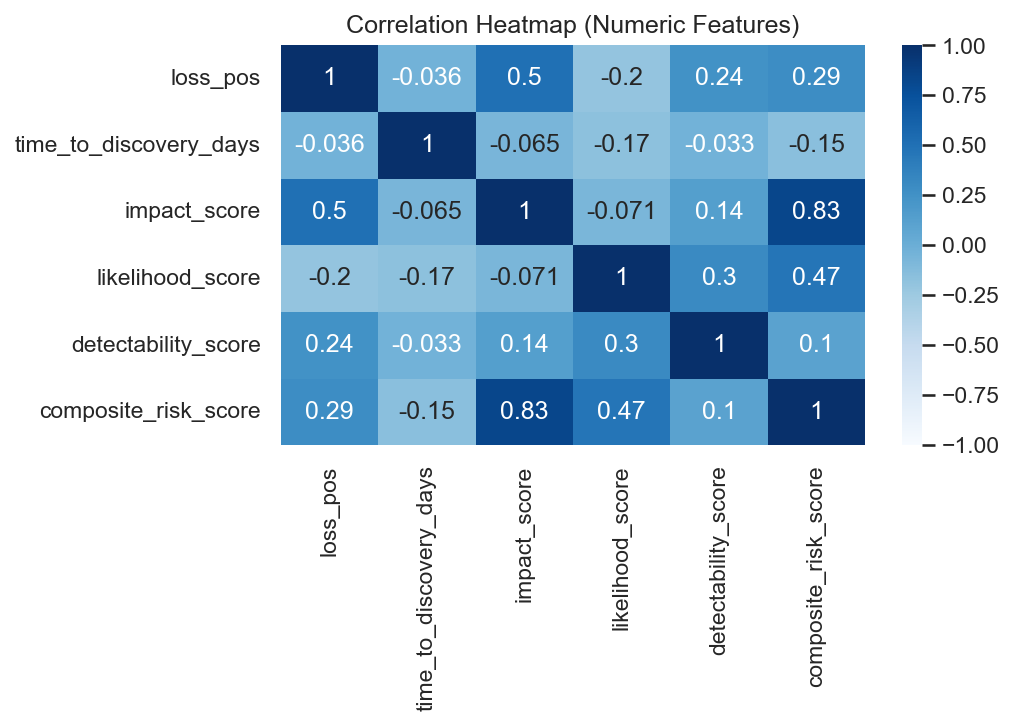
\includegraphics[width=0.5\textwidth]{../figure/Figure/figures_2/G1_correlation_heatmap.png}
\caption{Correlation heatmap of key variables: loss, risk scores, and time-to-discovery.}
\label{fig:correlation_heatmap}
\end{figure}

\subsection{Data Collection and Sources}
\label{sec:data_collection}

Our dataset comprises 649 blockchain security incident entries collected from multiple sources spanning 2016--early 2025. We employed a systematic approach to ensure comprehensive coverage while maintaining data quality and verifiability.

\begin{figure}[H]
    \centering
    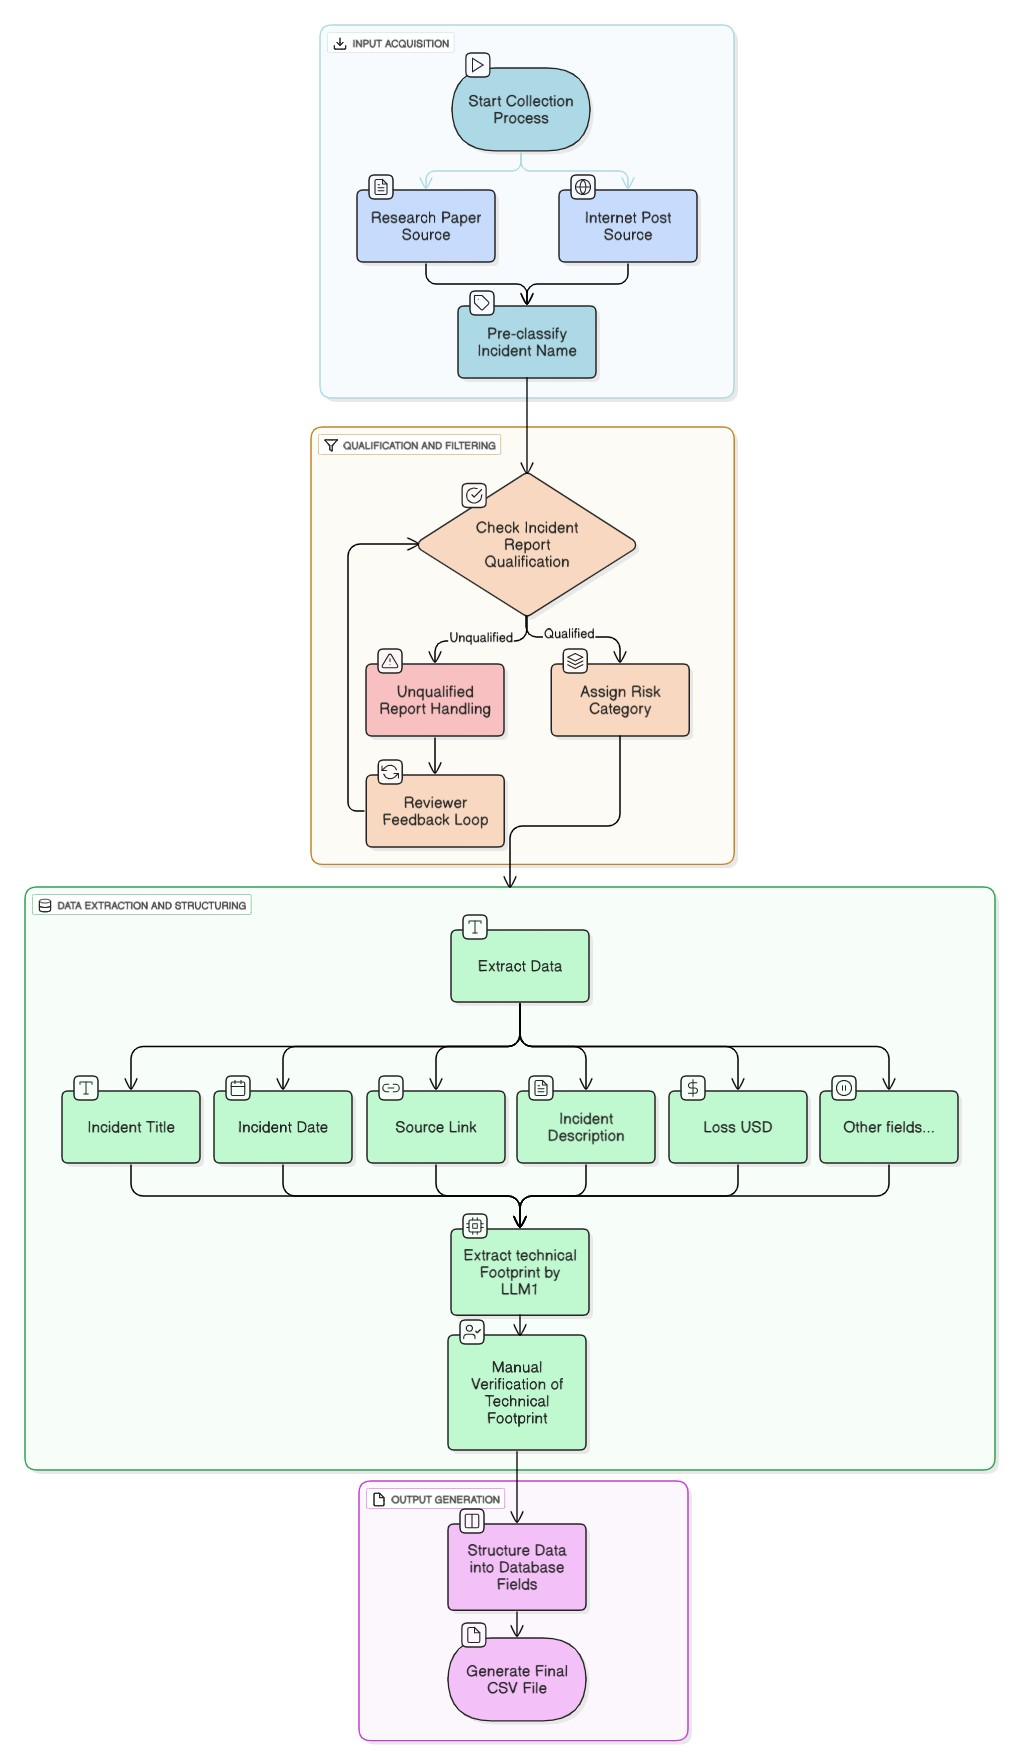
\includegraphics[width=0.4\textwidth]{../figure/methodology/collect_data.jpg}
    \caption{The process of collecting and reviewing data.}
    \label{fig:collect_data}
\end{figure}

\subsubsection{Primary Data Sources}
We collected incident data from the following primary sources:
\begin{itemize}
    \item \textbf{Web3IsGoingGreat:} A comprehensive database of blockchain security incidents with detailed incident reports and loss estimates
    \item \textbf{Rekt News:} Specialized platform tracking DeFi exploits and protocol vulnerabilities
    \item \textbf{Secureum:} Academic and industry reports on smart contract vulnerabilities and attacks
    \item \textbf{Chainalysis:} Blockchain analytics data for incident verification and impact assessment
    \item \textbf{Academic Literature:} Peer-reviewed papers and technical reports from security conferences
\end{itemize}

\subsubsection{Inclusion and Exclusion Criteria}
To ensure data quality and relevance, we applied the following criteria:

\textbf{Inclusion Criteria:}
\begin{itemize}
    \item Minimum financial loss of \$10,000 USD (adjusted for inflation)
    \item Verifiable incident reports with multiple independent sources
    \item Clear attribution to specific blockchain platforms or protocols
    \item Sufficient technical details to classify the attack vector
\end{itemize}

\textbf{Exclusion Criteria:}
\begin{itemize}
    \item Purely anecdotal or unverified reports
    \item Incidents with insufficient technical details for classification
    \item Non-blockchain related security incidents
    \item Duplicate reports of the same incident
\end{itemize}

\begin{figure}[H]
    \centering
    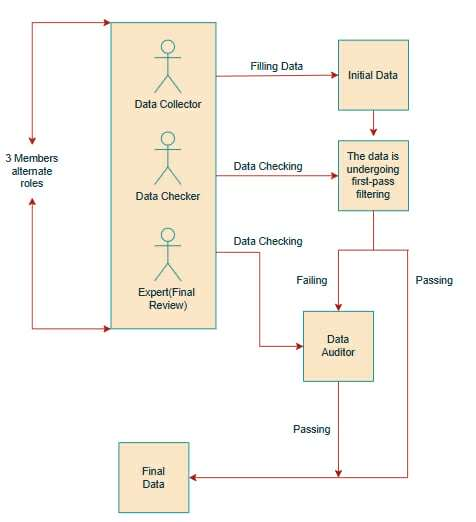
\includegraphics[width=0.4\textwidth]{../figure/methodology/peer_review.jpg}
    \caption{Peer-reviewing data.}
    \label{fig:peer_review}
\end{figure} 

\subsubsection{Data Collection Protocol}
Our data collection process followed a standardized protocol:
\begin{enumerate}
    \item \textbf{Source Identification:} Systematic review of primary and secondary sources
    \item \textbf{Initial Screening:} Application of inclusion/exclusion criteria
    \item \textbf{Data Extraction:} Structured extraction of incident details, financial impact, and technical characteristics
    \item \textbf{Verification:} Cross-referencing with multiple sources for accuracy
    \item \textbf{Quality Control:} Review by multiple team members for consistency
\end{enumerate}

\subsubsection{Dataset Schema and Dictionary}

The curated incident dataset contains 649 entries structured with 18 columns. Each row corresponds to a single classified incident with complete B-SAFE framework annotations:

\begin{itemize}
    \begin{figure}[H]
        \centering
        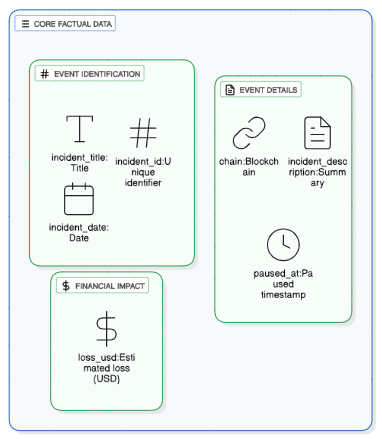
\includegraphics[width=0.3\textwidth]{../figure/methodology/core_factual_data.jpg}
        \caption{Core factual data of the dataset.}
        \label{fig:core_factual_data}
    \end{figure}
    \item \textbf{incident\_id}: Unique integer identifier for the security event
    \item \textbf{incident\_title}: Concise, descriptive title for the incident
    \item \textbf{incident\_date}: Date when the incident occurred or was first reported (MM/DD/YYYY format)
    \item \textbf{paused\_at}: Timestamp when a protocol was paused, if applicable
    \item \textbf{incident\_description}: Detailed text summary of the incident
    \item \textbf{loss\_usd}: Estimated financial loss in USD at the time of the incident
    \item \textbf{chain}: Primary blockchain or ecosystem affected (e.g., Ethereum, BNB Chain)
    \begin{figure}[H]
        \centering
        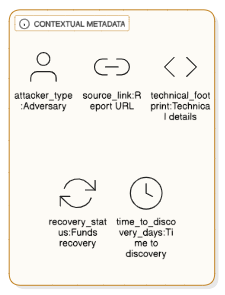
\includegraphics[width=0.3\textwidth]{../figure/methodology/contextual_metadata.jpg}
        \caption{Contextual metadata of the dataset.}
        \label{fig:contextual_data}
    \end{figure}
    \item \textbf{source\_link}: URL to a primary report or analysis of the incident
    \item \textbf{technical\_footprint}: JSON object containing structured technical details of the affected protocol, used for feature engineering
    \item \textbf{attacker\_type}: Classification of the adversary (e.g., Insider, External)
    \item \textbf{recovery\_status}: Status of the lost funds (e.g., Funds Lost, Funds Recovered)
    \item \textbf{time\_to\_discovery\_days}: Estimated time in days from exploit to public discovery
    \begin{figure}[H]
        \centering
        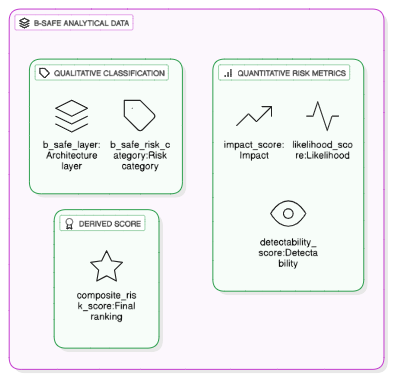
\includegraphics[width=0.3\textwidth]{../figure/methodology/analytical_data.jpg}
        \caption{Analytical data of the dataset.}
        \label{fig:analytical_data}
    \end{figure}
    \item \textbf{b\_safe\_layer}: Assigned B-SAFE architectural layer (NET, CON, SC, PRO, AUX)
    \item \textbf{b\_safe\_risk\_category}: Specific risk category identifier within the B-SAFE framework (e.g., SC-1, PRO-2)
    \item \textbf{impact\_score}: Assigned Impact (I) score on a 1-5 scale, as defined in Section IV.D
    \item \textbf{likelihood\_score}: Assigned Likelihood (L) score on a 1-5 scale, as defined in Section IV.D
    \item \textbf{detectability\_score}: Assigned Detectability (D) score on a 1-5 scale, as defined in Section IV.D
    \item \textbf{composite\_risk\_score}: Calculated priority ranking based on our formula
\end{itemize}

The dataset includes complete risk scoring for all 649 incidents, with 100\% coverage for impact, likelihood, and detectability scores, enabling comprehensive statistical analysis and validation of our risk quantification approach.

\begin{figure}[H]
\centering
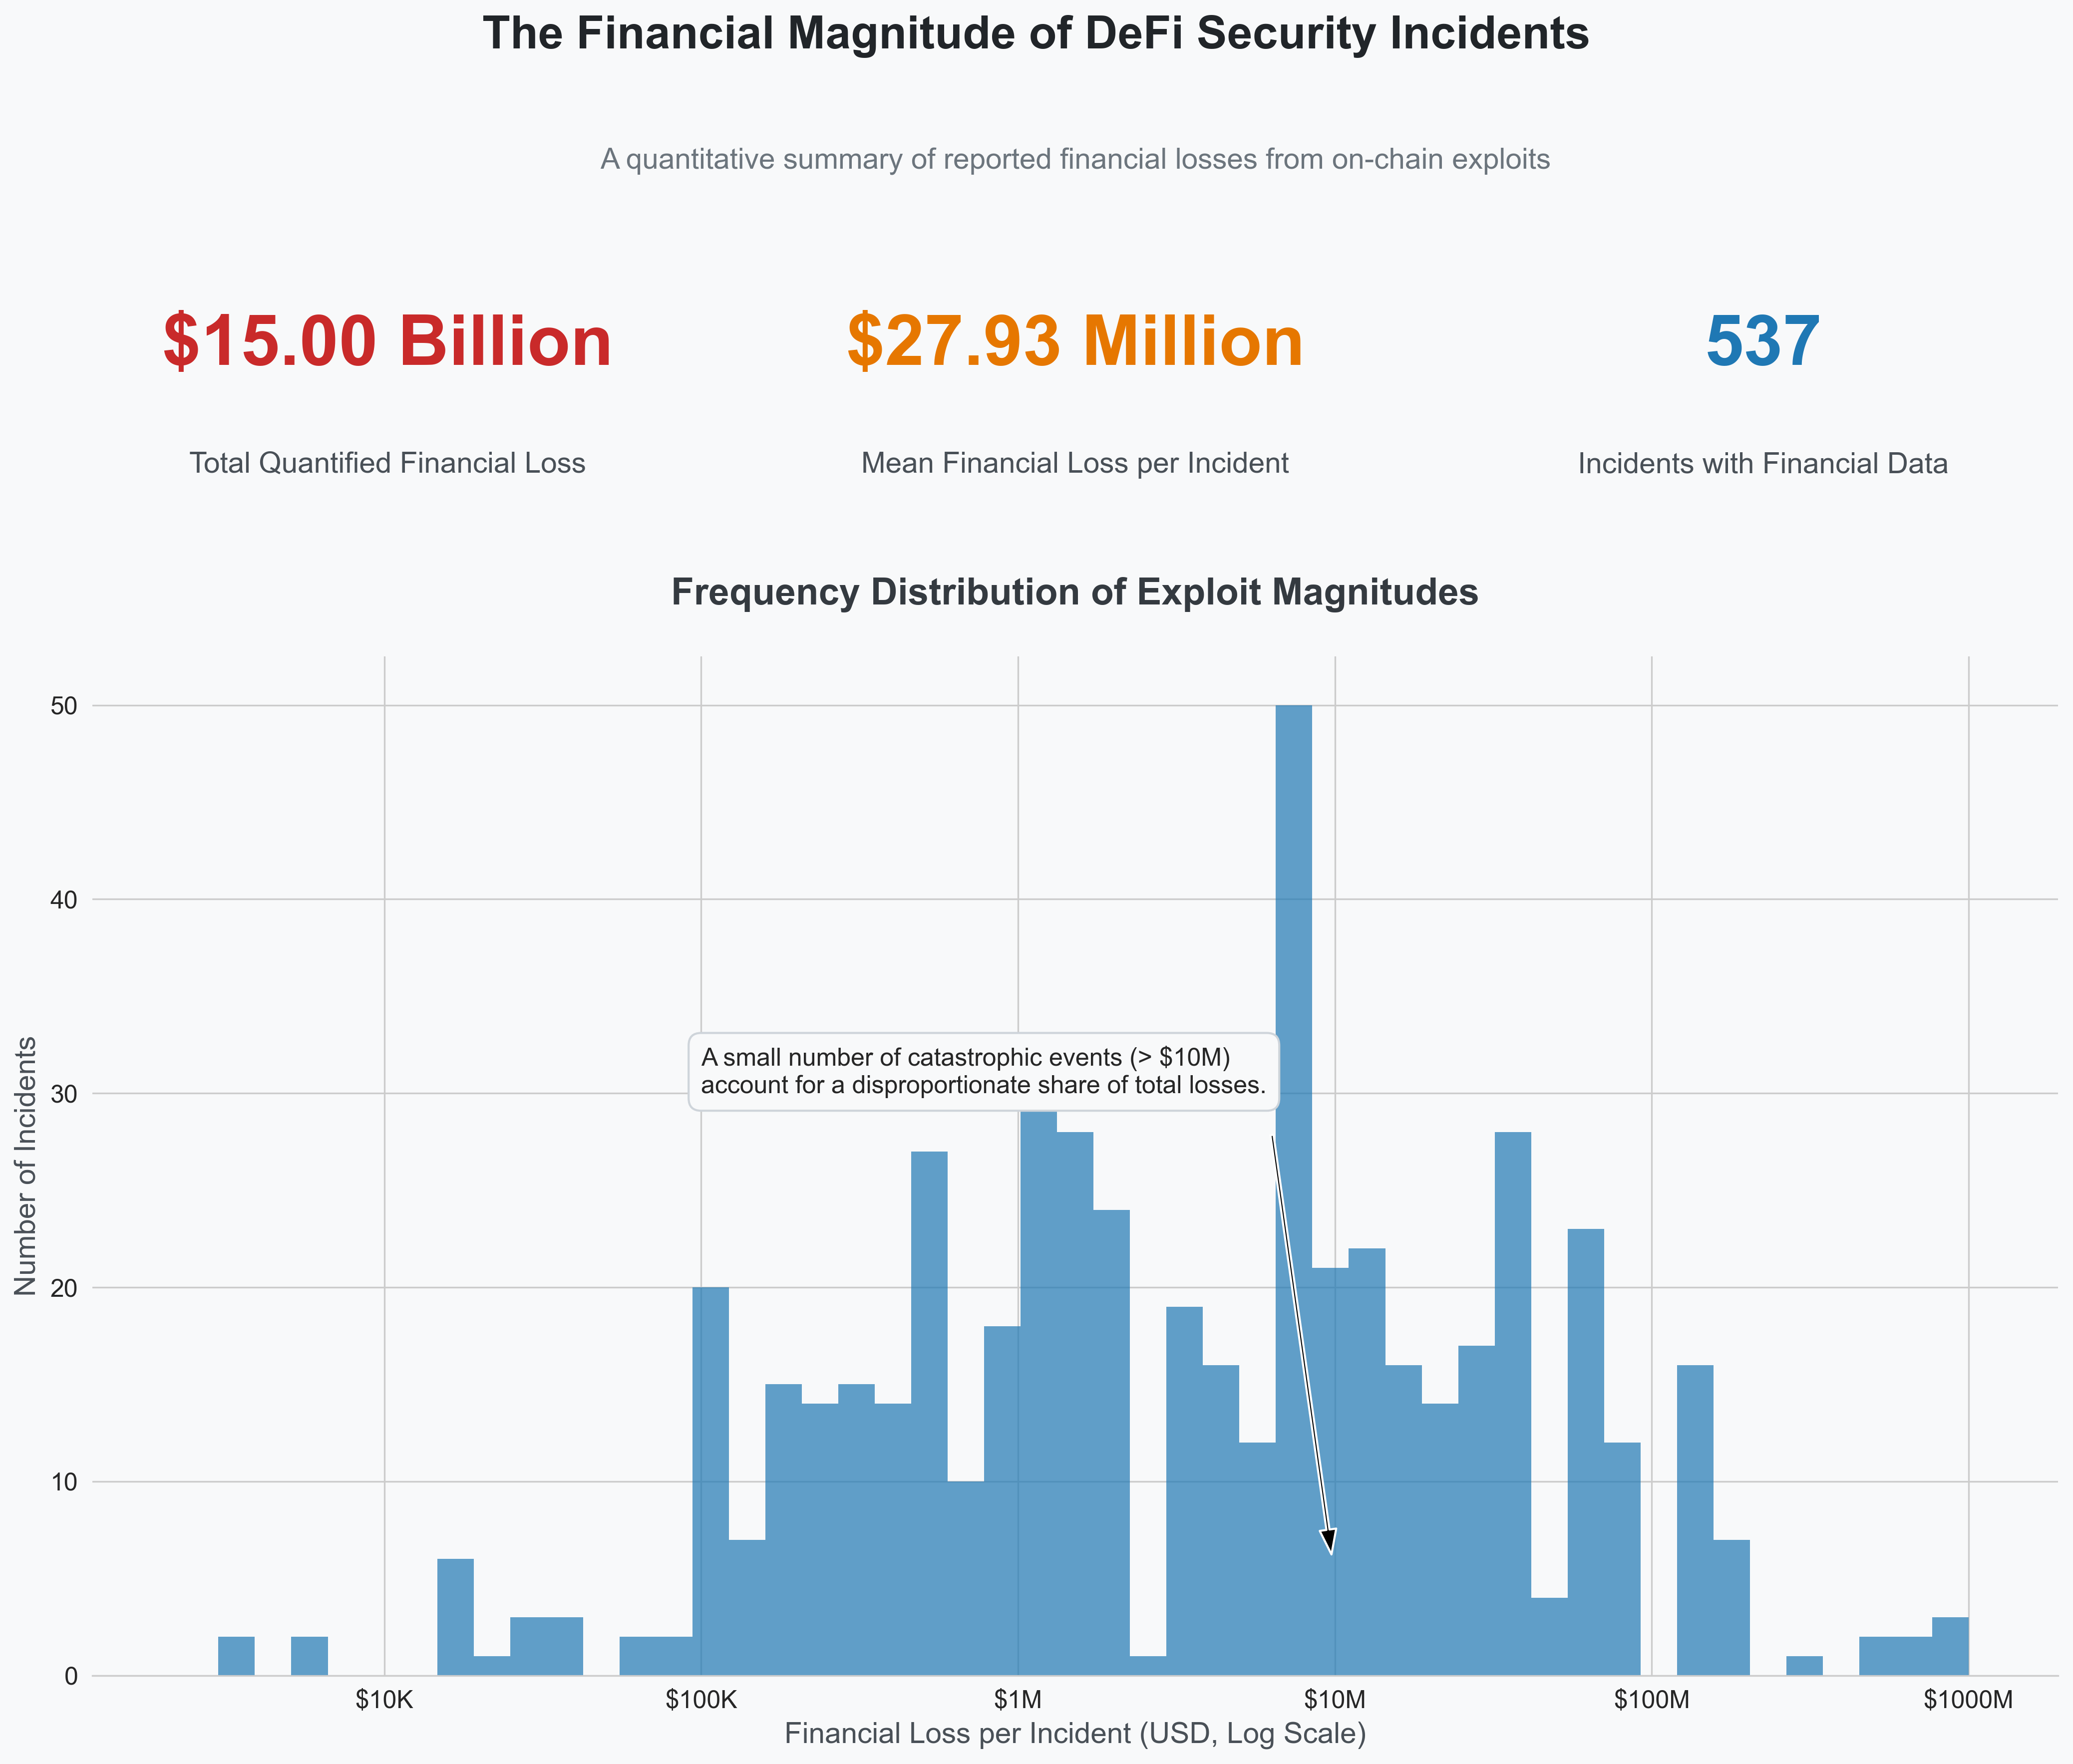
\includegraphics[width=0.5\textwidth]{../figure/methodology/fig4.png}
\caption{Financial Magnitude of DeFi Security Incidents}
\label{fig:data_pipeline}
\end{figure}

\subsection{Incident Labeling Protocol}
\label{sec:labeling_protocol}

To ensure consistent and reproducible classification of security incidents, we developed a comprehensive labeling protocol that maps each incident to our formal risk classification framework.

\subsubsection{Annotation Process}
Our labeling process involved multiple stages to ensure accuracy and consistency:

\begin{enumerate}
    \item \textbf{Initial Classification:} Each incident was initially classified by a primary annotator
    \item \textbf{Peer Review:} A second annotator reviewed and validated the classification
    \item \textbf{Expert Adjudication:} Disagreements were resolved through expert review
    \item \textbf{Quality Assurance:} Final classifications underwent quality control checks
\end{enumerate}

\subsubsection{Labeling Schema}
Each incident was labeled according to the following schema:

\textbf{Layer Classification (L):}
\begin{itemize}
    \item \textbf{NET:} Network layer attacks (eclipse, Sybil, partitioning)
    \item \textbf{CON:} Consensus layer attacks (51\%, selfish mining, rule violations)
    \item \textbf{SC:} Smart contract layer attacks (reentrancy, overflow, logic flaws)
    \item \textbf{PRO:} Protocol layer attacks (flash loans, oracle manipulation, governance)
    \item \textbf{AUX:} Auxiliary layer attacks (wallet security, key management, exchanges)
\end{itemize}

\textbf{Risk Category (R):} Each incident was assigned a unique risk category identifier (e.g., CON-1, SC-2)

\textbf{Preconditions (P):} Specific conditions that enabled the attack

\textbf{Invariants (I):} System invariants that were violated

\textbf{Controls (C):} Defense mechanisms that were present, absent, or insufficient

\subsubsection{Multi-Label Classification Rules}
For incidents spanning multiple layers or categories, we applied the following rules:
\begin{itemize}
    \item \textbf{Primary Classification:} Based on the initial attack vector
    \item \textbf{Secondary Classification:} For cascading effects across layers
    \item \textbf{Impact Weighting:} Consideration of financial and technical impact
\end{itemize}

\subsubsection{Example: Labeled Incident}
\textbf{Incident:} The DAO Hack (2016)
\begin{itemize}
    \item \textbf{Layer:} SC (Smart Contract)
    \item \textbf{Risk Category:} SC-1 (Reentrancy Attack)
    \item \textbf{Preconditions:} P1: Recursive call pattern, P2: State changes after external calls
    \item \textbf{Invariants:} INV-1: Value Conservation, INV-2: Access Control
    \item \textbf{Controls:} C1.1: Reentrancy guard (absent), C2.1: Checks-effects-interactions pattern (violated)
\end{itemize}

% TODO: Add inter-rater agreement statistics and validation procedures


\subsection{Feature Engineering}
\label{sec:feature_engineering}

To enable quantitative analysis and risk assessment, we constructed a comprehensive set of features from our incident dataset. These features capture both technical and economic aspects of each security incident.

\subsubsection{Financial Impact Features}
\textbf{Loss Normalization:}
\begin{itemize}
    \item \textbf{USD Value at Time of Incident:} All financial losses were converted to USD using exchange rates at the time of the incident
    \item \textbf{Inflation Adjustment:} Historical losses were adjusted for inflation using CPI data
    \item \textbf{Relative Loss:} Loss as a percentage of total value locked (TVL) or market capitalization
\end{itemize}

\textbf{Impact Categories:}
\begin{itemize}
    \item \textbf{Direct Losses:} Immediate financial impact on users and protocols
    \item \textbf{Indirect Losses:} Market cap reduction, loss of user confidence, regulatory costs
    \item \textbf{Recovery Costs:} Expenses related to incident response and remediation
\end{itemize}

\subsubsection{Technical Features}
\textbf{Attack Complexity:}
\begin{itemize}
    \item \textbf{Technical Sophistication:} Rated on a scale of 1-5 based on required expertise
    \item \textbf{Resource Requirements:} Computational, financial, or social engineering resources needed
    \item \textbf{Time to Exploit:} Duration from vulnerability discovery to successful exploitation
\end{itemize}

\textbf{Defense Effectiveness:}
\begin{itemize}
    \item \textbf{Audit Status:} Whether the affected system had undergone security audits
    \item \textbf{Control Implementation:} Presence and effectiveness of defense mechanisms
    \item \textbf{Detection Time:} Time between attack initiation and detection
\end{itemize}

\subsubsection{Temporal and Contextual Features}
\textbf{Timeline Features:}
\begin{itemize}
    \item \textbf{Incident Window:} Duration from attack initiation to resolution
    \item \textbf{Rescue Window:} Time available for emergency response and fund recovery
    \item \textbf{Market Conditions:} Cryptocurrency market state at time of incident
\end{itemize}

\textbf{Protocol Features:}
\begin{itemize}
    \item \textbf{Chain Affiliation:} Primary blockchain platform affected
    \item \textbf{Protocol Type:} DeFi protocol category (DEX, lending, yield farming, etc.)
    \item \textbf{Development Stage:} Protocol maturity and user adoption level
\end{itemize}

\subsubsection{Feature Validation}
To ensure feature quality and consistency:
\begin{itemize}
    \item \textbf{Cross-Validation:} Multiple sources were used to verify feature values
    \item \textbf{Expert Review:} Technical features were validated by security experts
    \item \textbf{Statistical Checks:} Outliers and anomalies were identified and investigated
\end{itemize}

% TODO: Add specific feature construction algorithms and data processing pipelines


\subsection{Risk Prioritization Approach}
\label{sec:risk_quantification}

We prioritize threats primarily by \textbf{Likelihood (L)} and \textbf{Impact (I)} on 1--5 scales. \textbf{Detectability (D)} is treated as a \textit{separate control-gap attribute} that influences monitoring and response planning rather than being combined arithmetically with L/I. This aligns with NIST/ISO practice, where detect functions mitigate but do not reduce inherent risk.

\subsubsection{Composite Score (L/I only)}
Where a single numeric priority is helpful, we use:
\begin{equation}
    \text{Composite} = (w_L \times L) + (w_I \times I),\quad w_L + w_I = 1
\end{equation}
with default weights $w_L=0.4$, $w_I=0.6$ to emphasize impact while preserving likelihood contributions. Detectability is reported alongside this composite.

\subsubsection{Weight Rationale}
The weights are selected to reflect established enterprise risk management principles where the magnitude of potential loss is the primary driver of priority. The assignment of $w_I=0.6$ and $w_L=0.4$ creates an \textit{impact-forward} model, ensuring that high-impact, low-likelihood "black swan" events are not unduly minimized in prioritization. This aligns with frameworks where impact asymmetries are a key consideration. While these weights are adaptable, they provide a stable baseline for triage. Future work could pursue formal weight calibration through expert elicitation methods (e.g., Delphi) on the incident corpus.

This weighting scheme aligns with industry best practices and reflects the asymmetric nature of blockchain security threats.

\subsubsection{Scoring Criteria}
\textbf{Likelihood (L) Scale:}
\begin{itemize}
    \item \textbf{1 (Very Low):} Theoretical attack, no known instances
    \item \textbf{2 (Low):} Rare occurrences, significant technical barriers
    \item \textbf{3 (Medium):} Occasional incidents, moderate technical requirements
    \item \textbf{4 (High):} Frequent occurrences, minimal technical barriers
    \item \textbf{5 (Very High):} Widespread exploitation, automated tools available
\end{itemize}

\textbf{Impact (I) Scale:}
\begin{itemize}
    \item \textbf{1 (Minimal):} < \$100K loss, no service disruption
    \item \textbf{2 (Minor):} \$100K-\$1M loss, temporary service issues
    \item \textbf{3 (Moderate):} \$1M-\$10M loss, significant service disruption
    \item \textbf{4 (Major):} \$10M-\$100M loss, protocol failure
    \item \textbf{5 (Critical):} > \$100M loss, systemic failure
\end{itemize}

\textbf{Detectability (D) Scale:}
\begin{itemize}
    \item \textbf{1 (Very Easy):} Immediate detection, clear indicators
    \item \textbf{2 (Easy):} Quick detection, obvious symptoms
    \item \textbf{3 (Moderate):} Detectable with monitoring, some ambiguity
    \item \textbf{4 (Difficult):} Requires specialized tools, subtle indicators
    \item \textbf{5 (Very Difficult):} Stealth attacks, minimal indicators
\end{itemize}

\subsubsection{Sensitivity Analysis}
We examine ranking stability across reasonable $w_L/w_I$ variations and confirm that categories with high impact remain top priorities. Full quantitative evaluation is future work.

\subsection{Tools and Reproducibility}
\label{sec:tools_and_reproducibility}

To ensure the reproducibility of our analysis and enable future research, we have developed a comprehensive toolkit and documented our methodology in detail.

\subsubsection{Data Processing Pipeline}
Our data processing pipeline consists of several interconnected components:

\textbf{Data Collection Tools:}
\begin{itemize}
    \item \textbf{Web Scrapers:} Automated tools for collecting incident data from primary sources
    \item \textbf{API Integrations:} Direct access to blockchain analytics and incident databases
    \item \textbf{Manual Review Interface:} Structured forms for expert annotation and validation
\end{itemize}

\textbf{Data Processing Scripts:}
\begin{itemize}
    \item \textbf{Data Cleaning:} Python scripts for removing duplicates and standardizing formats
    \item \textbf{Feature Extraction:} Automated extraction of technical and financial features
    \item \textbf{Quality Control:} Validation scripts for ensuring data consistency
\end{itemize}

\subsubsection{Analysis Framework}
Our analysis framework provides standardized tools for incident organization and risk assessment consistent with a checklist-first approach:

\textbf{Classification Tools:}
\begin{itemize}
    \item \textbf{Checklist Tagging Scripts:} Lightweight scripts to assist manual labeling and consistency checks
    \item \textbf{Risk Calculator:} Implementation of our risk scoring formula (spreadsheet and script variants)
    \item \textbf{Visualization Suite:} Tools for generating heatmaps, timelines, and summary plots
\end{itemize}

\textbf{Validation Framework:}
\begin{itemize}
    \item \textbf{Dual-Review:} Peer review of labels with adjudication for disagreements
    \item \textbf{Expert Review Interface:} Tools for manual validation and correction
    \item \textbf{Audit Trail:} Change logs and evidence links for checklist items
    \item \textbf{Model Evaluation (Planned):} Train/test splits with accuracy, precision/recall/F1 for classifier; $R^2$ and MSE for regressors; calibration curves and confusion matrices.
\end{itemize}

\subsubsection{Reproducibility Package}
To enable full reproducibility, we provide:

\textbf{Artifacts:}
\begin{itemize}
    \item \textbf{Version Control:} Git repository for LaTeX sources, labeling schema, and helper scripts
    \item \textbf{Dependencies:} Minimal environment for reproducing figures and tables
\end{itemize}

\textbf{Documentation:}
\begin{itemize}
    \item \textbf{API Documentation:} Complete documentation for all tools and functions
    \item \textbf{Tutorials:} Step-by-step guides for reproducing our analysis
    \item \textbf{Example Notebooks:} Jupyter notebooks demonstrating key analyses
\end{itemize}

\subsubsection{Software Versions and Dependencies}
Our analysis and pipeline were implemented with the following stack:
\begin{itemize}
    \item \textbf{Python 3.9+:} Core scripting and analysis
    \item \textbf{Pandas 1.5+:} Data manipulation
    \item \textbf{NumPy 1.21+:} Numerical computing
    \item \textbf{XGBoost 1.7+:} Risk regressors and category classifiers
    \item \textbf{Scikit-learn 1.1+:} Preprocessing and calibration
    \item \textbf{Matplotlib 3.5+:} Visualization
\end{itemize}

% Consolidated into Section IV-F Limitations

\subsection{Limitations}
\label{sec:limitations}

While our methodology provides a comprehensive framework for blockchain security assessment, we acknowledge several limitations that may affect the completeness and accuracy of our analysis.

\subsubsection{Data Completeness}
\textbf{Reporting Bias:}
\begin{itemize}
    \item \textbf{Underreporting:} Many incidents may go unreported, particularly smaller attacks or those affecting less prominent protocols
    \item \textbf{Selective Reporting:} Incidents may be reported differently based on their impact, perpetrator identity, or media attention
    \item \textbf{Geographic Bias:} Incidents in certain regions may be underrepresented due to language barriers or reporting infrastructure
\end{itemize}

\textbf{Verification Challenges:}
\begin{itemize}
    \item \textbf{Anonymous Nature:} Blockchain's pseudonymous nature makes it difficult to verify all incident details
    \item \textbf{Cross-Chain Complexity:} Multi-chain attacks may be undercounted or misclassified
    \item \textbf{Time Delays:} Some incidents may take time to be discovered and reported
\end{itemize}

\subsubsection{Methodological Limitations}
\textbf{Classification Accuracy:}
\begin{itemize}
    \item \textbf{Inter-Rater Reliability:} Despite our multi-stage review process, some classification decisions may be subjective
    \item \textbf{Evolution of Attacks:} New attack vectors may not fit neatly into our existing classification schema
    \item \textbf{Multi-Vector Attacks:} Complex attacks spanning multiple layers may be difficult to classify accurately
\end{itemize}

\textbf{Risk Assessment Challenges:}
\begin{itemize}
    \item \textbf{Historical Bias:} Our risk scoring may be influenced by historical patterns that may not predict future threats
    \item \textbf{Context Dependence:} Risk levels may vary significantly based on specific protocol implementations
    \item \textbf{Adaptive Adversaries:} Attackers may adapt their strategies in response to improved defenses
\end{itemize}

\subsubsection{Technical Limitations}
\textbf{Data Quality:}
\begin{itemize}
    \item \textbf{Incomplete Information:} Some incidents lack sufficient technical details for comprehensive analysis
    \item \textbf{Inconsistent Reporting:} Different sources may report the same incident with varying levels of detail
    \item \textbf{Verification Gaps:} Not all reported incidents can be independently verified
\end{itemize}

\textbf{Analysis Scope:}
\begin{itemize}
    \item \textbf{Platform Coverage:} Our analysis focuses on major blockchain platforms and may miss emerging ecosystems
    \item \textbf{Temporal Scope:} The 2017-2024 timeframe may not capture the full evolution of blockchain security threats
    \item \textbf{Protocol Types:} Certain protocol categories may be overrepresented in our dataset
\end{itemize}

\subsubsection{External Validity}
\textbf{Generalizability:}
\begin{itemize}
    \item \textbf{Protocol-Specific Factors:} Our findings may not generalize to all blockchain protocols
    \item \textbf{Market Conditions:} Analysis during specific market conditions may not reflect long-term trends
    \item \textbf{Regulatory Environment:} Changes in regulatory landscape may affect attack patterns and reporting
\end{itemize}

\textbf{Future Applicability:}
\begin{itemize}
    \item \textbf{Technology Evolution:} Rapid technological changes may render some of our findings obsolete
    \item \textbf{Emerging Threats:} New attack vectors may emerge that are not captured in our current framework
    \item \textbf{Defense Evolution:} Improved security practices may change the effectiveness of existing attack vectors
\end{itemize}

\subsubsection{Mitigation Strategies}
To address these limitations, we have implemented several mitigation strategies:
\begin{itemize}
    \item \textbf{Multiple Data Sources:} Cross-validation across multiple sources to reduce reporting bias
    \item \textbf{Expert Review:} Regular review by security experts to validate classifications
    \item \textbf{Continuous Updates:} Framework designed for ongoing updates as new threats emerge
    \item \textbf{Transparency:} Full disclosure of methodology and limitations to enable critical evaluation
\end{itemize}

% TODO: Add specific examples of limitations and their potential impact on results

